\documentclass[11pt,a4paper]{article}
\usepackage[left=22mm,right=22mm,top=24mm,bottom=27mm,footskip=12mm]{geometry}
\usepackage[T1]{fontenc}
\usepackage{newtxtext}
\usepackage{amsmath,amsthm,mathtools,newtxmath}
\usepackage{microtype,graphicx,booktabs,array,tabularx,multirow,makecell,enumitem,float,placeins}
\usepackage{xcolor,listings,caption,subcaption,titlesec,fancyhdr}
\usepackage[colorlinks=true,urlcolor=accent,linkcolor=ink,bookmarksnumbered=true,pdfpagemode=UseOutlines,pdftitle={Appendix — Research Extensions},pdfsubject={Project 3H. Three extensions of the coursework predator–prey model}]{hyperref}
\usepackage{bookmark}
\definecolor{ink}{HTML}{152D3A}
\definecolor{accent}{HTML}{195569}
\definecolor{faint}{HTML}{E3ECEE}
\definecolor{soft}{HTML}{F4F7F8}
\setlength{\parindent}{0pt}
\setlength{\parskip}{4pt plus 1pt minus 1pt}
\setlist{topsep=3pt,itemsep=2pt,parsep=0pt}
\titleformat{\section}{\Large\bfseries\color{ink}}{\thesection}{.5em}{}
\titleformat{\subsection}{\large\bfseries\color{accent}}{\thesubsection}{.5em}{}
\titleformat{\subsubsection}{\normalsize\bfseries\color{ink}}{\thesubsubsection}{.5em}{}
\titlespacing*{\section}{0pt}{0pt plus 2pt}{8pt}
\titlespacing*{\subsection}{0pt}{10pt plus 2pt}{4pt}
\titlespacing*{\subsubsection}{0pt}{7pt plus 2pt}{2pt}
\captionsetup{hypcap=false,font=small,labelfont=bf,justification=raggedright,singlelinecheck=false,skip=5pt}
\lstset{basicstyle=\small\ttfamily,keywordstyle=\bfseries\color{accent},commentstyle=\color{gray},showstringspaces=false,breaklines=true,columns=fullflexible,keepspaces=true,backgroundcolor=\color{soft},frame=single,framerule=.35pt,rulecolor=\color{faint},framesep=4pt,xleftmargin=5pt,xrightmargin=5pt,aboveskip=6pt,belowskip=6pt}
\pagestyle{fancy}\fancyhf{}
\fancyfoot[R]{\small\sffamily\thepage}
\renewcommand{\headrulewidth}{0pt}
\setlength{\emergencystretch}{1.5em}
\raggedbottom
\newcommand{\startdirection}[2]{%
  \clearpage
  \pdfbookmark[0]{Direction #1. #2}{direction-#1}\phantomsection\label{start:#1}%
  \setcounter{equation}{0}\setcounter{figure}{0}\setcounter{table}{0}%
  \renewcommand{\theequation}{#1.\arabic{equation}}%
  \renewcommand{\thefigure}{#1.\arabic{figure}}\renewcommand{\thetable}{#1.\arabic{table}}%
  \renewcommand{\theHequation}{d#1.\arabic{equation}}%
  \renewcommand{\theHfigure}{d#1.\arabic{figure}}\renewcommand{\theHtable}{d#1.\arabic{table}}%
}
\begin{document}
\pdfbookmark[0]{Appendix — Research Extensions}{appendix-home}
{\fontsize{25}{28}\selectfont\bfseries\color{ink}Appendix --- Research Extensions\par}
\vspace{3pt}
The three studies use the same coursework equation as their starting point. Each chapter pairs its results with figures, mathematical proofs, Python code, and Lean verification.\par
\vspace{4pt}
\noindent\textbf{1. How does the feeding law change coexistence?}\par
We kept the coursework's weak Allee prey growth and changed only the feeding law. All five models preserve positive populations and keep them bounded. In the two prey-dependent models (P1 and P2), positive coexistence fixes prey density independently of carrying capacity. The original foraging-arena response (P0) can support two attracting coexistence states. With ratio-dependent feeding (P4), enrichment lowers the Jacobian trace at every positive coexistence state with positive determinant for the coursework growth law. For a positive growth factor $g$ with $g'>0$, the same decrease holds at a given prey density for every admissible ratio-dependent intake if and only if $(1/g)''\geq0$ there.

\medskip
\noindent\textbf{2. How do prey growth and predator competition interact?}\par
We kept the feeding law fixed and paired three prey growth laws with and without direct predator competition. Logistic growth allows at most one positive equilibrium. Weak and strong Allee growth can each support three. When the three growth laws are calibrated to the same coexistence state at zero competition, positive competition orders predator density along their common branches with positive determinant. Predator density is highest for strong Allee growth, intermediate for weak Allee growth, and lowest for logistic growth. This ranks equilibrium levels even when predator density falls in all three models. In 48 disturbance simulations at the study baseline, 45 recovered. All three failures followed prey removal under strong Allee growth.

\medskip
\noindent\textbf{3. What transfers when the same equation is fitted to other systems?}\par
We kept the ecological equation and fitted its coefficients to training conditions in tumor--T-cell and bacteria--phage datasets. The equation had lower mean held-out error than the CARRGO model on the PBT138 cell line, while the infection-stage model had lower four-hour error in 11 of 12 $\lambda$-phage conditions. In 12 held leukemia conditions, fitting targets alone predicted none of the observed early T-cell increases. Fitting both populations predicted all 12, but mean target root-mean-square error rose from 81,634 to 197,580 cells. The measured trade-off concerns predictions for held conditions from this dataset.

\vfill
{\small\sffamily\color{accent}\textbf{Full results, figures, proofs, and verification}\par}
\vspace{3pt}
{\small\hyperref[start:1]{Direction 1\quad Predation mechanisms}\dotfill\pageref{start:1}\par
\hyperref[start:2]{Direction 2\quad Growth and competition}\dotfill\pageref{start:2}\par
\hyperref[start:3]{Direction 3\quad Cross-domain prediction}\dotfill\pageref{start:3}\par}
\startdirection{1}{Predation mechanisms and enrichment}
\section*{Direction 1. How the feeding law changes coexistence and enrichment}

\subsection*{Abstract}
We kept the coursework prey growth law and compared five ways predators consume prey. In all five models, positive initial populations remain positive and ultimately bounded. The feeding laws differ in how many coexistence equilibria they admit and how those equilibria respond to increasing carrying capacity. For prey-dependent feeding, a feasible predator break-even density gives a unique coexistence branch and an upward stability crossing as carrying capacity increases. Predator interference can give three equilibria. For ratio-dependent feeding, we prove a necessary and sufficient condition on prey growth for enrichment to decrease the equilibrium trace across all admissible intakes. In four algae--rotifer experiments, the best one-step predictor changed when the fitting bounds were widened.

\subsection*{Results}
Let $x$ and $y$ be prey and predator density, $K$ the prey carrying capacity, $e$ the conversion efficiency, and $d$ the predator mortality rate. The original equations are
\[
 \dot x=xq(x,K)-P(x,y),\qquad \dot y=eP(x,y)-dy,\qquad
 q(x,K)=r(1-x/K)(1+\alpha x).
\]
All shared coefficients $r,K,\alpha,e,d$ are positive. The weak Allee factor $1+\alpha x$ acts on prey growth. The per-capita growth rate rises near zero precisely when $\alpha K>1$. The coursework uses $P_0=mxy/(\beta+y)$, equivalently $axy/(1+cy)$ with $a=m/\beta$ and $c=1/\beta$.

\begin{center}\small
\begin{tabular}{@{}lll@{}}
\toprule
Model & Total consumption $P(x,y)$ & What fixes positive coexistence \\
\midrule
P0\quad Foraging arena & $axy/(1+cy)$ & An affine predator nullcline \\
P1\quad Mass action & $axy$ & A fixed prey density \\
P2\quad Holling type II & $axy/(1+bx)$ & A fixed prey density \\
P3\quad Beddington--DeAngelis & $axy/(1+bx+cy)$ & An affine predator nullcline \\
P4\quad Ratio-dependent Holling II & $axy/(x+cy)$ & A fixed predator-to-prey ratio \\
\bottomrule
\end{tabular}
\end{center}

For P0--P3, let $\mathcal R=eaK/[d(1+bK)]$, with $b=0$ where absent. When $\mathcal R\leq1$, every positive trajectory converges to $(K,0)$. When $\mathcal R>1$, both species persist uniformly. In this regime P1/P2 have one positive equilibrium. P2 requires $ea>db$ for a finite positive break-even density. P0/P3 can have three, with a saddle between the outer branches. For example, P0 with $r=e=d=1$, $K=8$, $\alpha=1/2$, $a=9/2$, and $c=8/3$ has attracting equilibria $(1,21/16)$ and $(3,75/16)$ separated by the saddle $(2,3)$. P4 has at most two positive equilibria. A positive predator invasion rate at $(K,0)$ can coexist with an open basin of joint extinction.

When $\alpha>0$ and $u=1/(ea/d-b)>0$, the P1/P2 coexistence branch exists for $K>u$. Increasing $K$ carries this branch through a supercritical Hopf bifurcation, creating nearby stable oscillations. For P4 the trace decreases on every positive-determinant branch under the same prey growth. P0 and P3 each allow either trace direction. Separate exact examples give fold, Hopf and Bogdanov--Takens bifurcations in P0, P3, and P4. A Bogdanov--Takens point has a double zero eigenvalue and two independent unfolding parameters. For example, P0 has a supercritical Hopf bifurcation at $(1,1)$ when $(r,K,\alpha,a,c)=(9/25,6,7/3,2,1)$ and $e=d=1$. At this point $\Delta=1/4$ and, as $r$ varies, $dT/dr=-1/6$.

\clearpage
\subsection*{Figures and tables}
\textbf{A controlled comparison.}
We matched the intake of a rare predator at $x=10$ to $0.9$ in all five laws. The common parameters were $(r,K,\alpha,e,d)=(0.7,10,0.12,0.6,0.3)$. For P0--P3, $b=0.15$ and $c=0.2$ where present and $a=0.09(1+10b)$. For P4, $a=0.9$ and $c=2$. This specifies the same invasion rate at the reference capacity while allowing distinct responses away from it.

\begin{center}
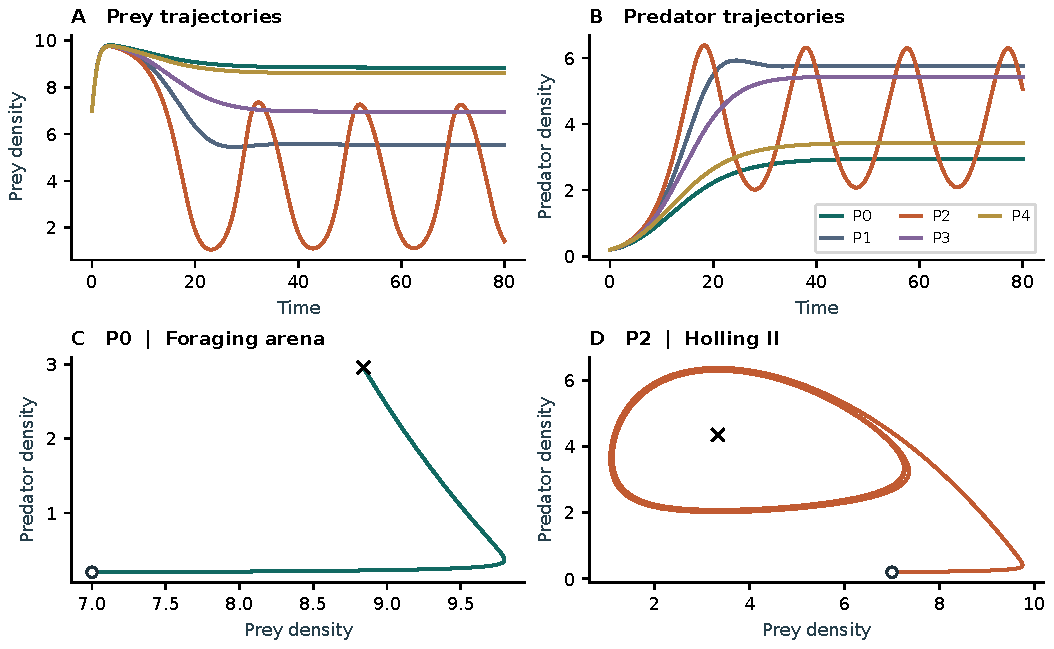
\includegraphics[width=.91\linewidth]{d1/figures/matched_dynamics.pdf}
\end{center}
{\small\textbf{Figure 1.1.} All trajectories start at $(7,0.2)$. The top panels track densities over time. The lower panels trace P0 and P2 in the population plane. The cross marks coexistence. P0 approaches its equilibrium, whereas P2 oscillates around an unstable equilibrium.}

\begin{center}\small
\begin{tabular}{@{}lrrrrr@{}}
\toprule
 & \multicolumn{3}{c}{Matched synthetic comparison} & \multicolumn{2}{c}{Observed one-step error}\\
\cmidrule(lr){2-4}\cmidrule(l){5-6}
Model & $x_*$ & $y_*$ & Largest $\operatorname{Re}\lambda$ & Primary bounds & Wider bounds\\
\midrule
P0 & 8.841 & 2.957 & $-0.1416$ & 0.867367 & \textbf{0.868031}\\
P1 & 5.556 & 5.761 & $-0.2204$ & 0.906098 & 0.906096\\
P2 & 3.333 & 4.356 & $+0.0389$ & 0.906112 & 0.906097\\
P3 & 6.958 & 5.437 & $-0.2615$ & 0.867378 & 0.868132\\
P4 & 8.593 & 3.437 & $-0.1506$ & \textbf{0.857747} & 0.870391\\
Last observation & & & & 1.040276 & 1.040276\\
\bottomrule
\end{tabular}
\end{center}
{\small\textbf{Table 1.1.} The last two columns use four observed algae--rotifer chemostat experiments (\href{https://doi.org/10.1038/s41586-019-1857-0}{Blasius et al.}, \textit{Nature} 577, 226--230, 2020). Each experiment was held out in turn, giving 861 observed intervals. Each prediction started from the latest observed populations. We averaged prey and predator errors after scaling by training variation, then weighted the four experiments equally. Smaller scores are better. Widening every parameter range tenfold at both ends changed the best mean score from P4 to P0. These data leave the feeding law unresolved.}

\clearpage
\textbf{Two local stability crossings.}
The following example uses $g(x)=1+x^2$ in $q(x,K)=g(x)(1-x/K)$ to explore what can happen outside the coursework growth law. Fix $e=d=1$ and $p(z)=110/(65+54z)$, where $z=y/x$. Its unique positive branch satisfies
\[
 y=\tfrac56x,\quad
 K=\frac{6x(1+x^2)}{1+6x^2},\quad
 T=-\frac{(3x^2-1)(4x^2-1)}{12(1+x^2)},\quad
 \Delta=\tfrac{3}{88}-\tfrac{9}{22}T.
\]
Here $T$ is the Jacobian trace and $\Delta$ its determinant. Both $K'(x)$ and $\Delta$ are positive along the branch. Thus the signs of the two trace factors give the stability intervals directly.

\begin{center}
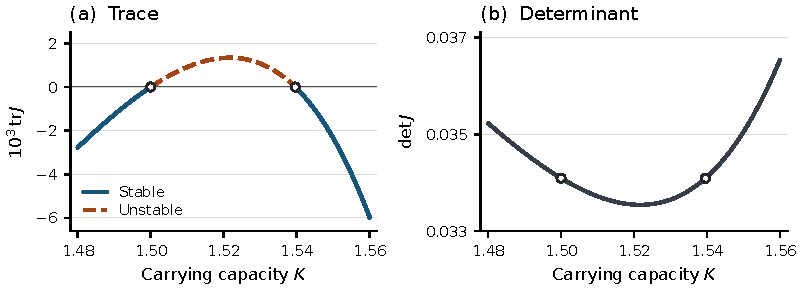
\includegraphics[width=.89\linewidth]{d1/figures/stability_crossing.pdf}
\end{center}
{\small\textbf{Figure 1.2.} With the same intake throughout, coexistence loses local stability at $K=3/2$ and regains it at $K=8/(3\sqrt3)$. The corresponding trace slopes are $1/9$ and $-3\sqrt3/32$. A Hopf classification for these two crossings requires the nonlinear coefficient.}

\medskip\noindent\textbf{Two long-term outcomes under one parameter set.}
Return to P4 with the coursework factor $g=1+x/2$. Set $K=8$, $a=4/5$, $c=8/15$, $e=1$, and $d=1/5$. The prey coordinates of the two positive equilibria are $3\pm\sqrt7$. The lower equilibrium is a saddle and the upper one attracts nearby trajectories.

\begin{center}
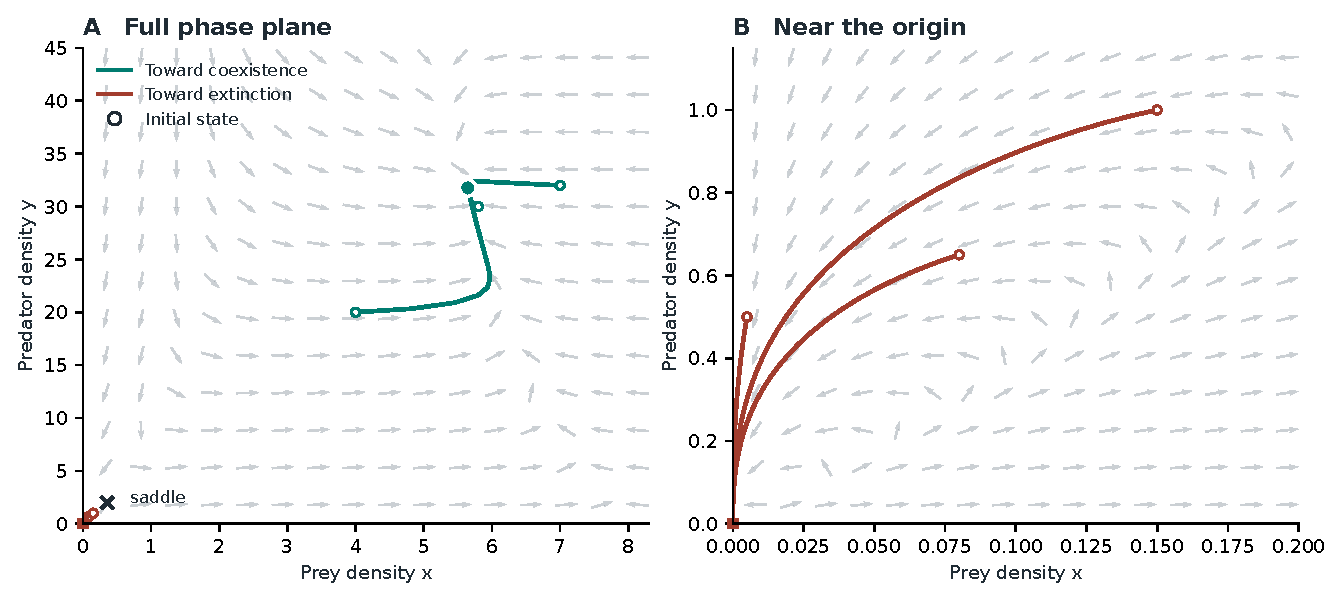
\includegraphics[width=.86\linewidth]{d1/figures/ratio_basins.pdf}
\end{center}
{\small\textbf{Figure 1.3.} Three initial conditions approach coexistence and three approach joint extinction. In the region $0<x<0.01$, $u=8y/(15x)>10$, the equations give $\dot x/x<-0.35$ and $\dot u/u>0.23$. This region is forward invariant. There $x\to0$, $u\to\infty$ and $\dot y/y\to-0.2$, proving convergence to extinction for an open set of initial states.}

\clearpage
\subsection*{Mathematical proofs}
\textbf{Why the five laws give different equilibrium counts.}
For P0--P3 write $D=1+bx+cy$, putting absent coefficients equal to zero, and set $A=ea/d-b$. Predator break-even at a positive equilibrium gives $1+cy=Ax$. The prey equation then gives $y=exq/d$. Thus P1/P2 fix $x=1/A$ when $A>0$ and $K>1/A$. P0/P3 require a root of the cubic
\[
 H(x)=\frac{ce}{d}xq(x,K)-Ax+1=0,\qquad 1/A<x<K.
\]
For the P0 example above, $H=-(x-1)(x-2)(x-3)/6$. At positive roots $\Delta=-dqxH'/D$. The middle root has negative determinant, while the two outer roots have positive determinant and negative trace by substitution. In P4 the same predator equation fixes $\rho=y/x=(ea/d-1)/c$. The prey equation reduces to $q(x,K)=\rho d/e$, a quadratic level equation. The common identity $(ex+y)'=exq-dy$ explains the shared bound despite these different geometries. For any $0<\eta\le d$, $(ex+y)'+\eta(ex+y)\le ex(q+\eta)$, whose supremum over $x\ge0$ is finite.

\medskip\noindent\textbf{Reciprocal-curvature theorem.}
Fix $e,d>0$ and a prey density $s$ in an open interval $I\subset(0,\infty)$. Let $g\in C^2(I)$ with $g,g'>0$. Consider the original-time system
\[
 \dot x=xg(x)(1-x/K)-yp(y/x),\qquad \dot y=y[ep(y/x)-d].
\]
The condition $(1/g)''(s)\ge0$ is equivalent to the following property. For every positive, strictly decreasing $p\in C^1(0,\infty)$, every $K_0>0$, and every $v>0$ giving an equilibrium $(s,v)$ with $\Delta>0$ at $K_0$, the trace along its local branch satisfies $dT/dK<0$ at $K_0$. Only $K$ varies on a given branch.

\medskip\noindent\textit{Proof.}
At coexistence $p(\rho)=d/e$, so $\rho$ and $Q=\rho d/e$ are fixed and $q(x,K)=Q$. Direct differentiation of the original field gives
\[
 T=xq_x+Q+\rho(\rho+e)p'(\rho),\qquad
 \Delta=e\rho p'(\rho)xq_x .
\]
Strict decrease gives $p'(\rho)\le0$. A positive determinant forces $p'(\rho)<0$ and $q_x<0$, so $x_K=-q_K/q_x>0$ by implicit differentiation. Put $E=xg'/g$, $D_0=g-(1+E)Q$, and $U=g/(1+E)$. Substituting $x/K=1-Q/g$ gives $xq_x=-D_0$. Thus $0<Q<U$ and
\[
 T_K=x_KL(Q),\qquad L(Q)=QE'-g',\qquad
 L(0)=-g',\quad L(U)=-\frac{s g^2}{1+E}(1/g)''(s).
\]
The endpoint expressions use $x=s$. If reciprocal curvature is nonnegative, the affine function $L$ is negative at $0$ and nonpositive at $U$, hence strictly negative throughout the open interval. Conversely, when curvature is negative, $L$ has an interior zero and takes both signs. To realize any interior load, choose $\rho=eQ/d$, $K_0=s/(1-Q/g(s))$, and $p(z)=(2d/e)/(1+z/\rho)$. Then $q(s,K_0)=Q$, $p(\rho)=d/e$, $p'(\rho)<0$, and $D_0>0$. These choices yield $\Delta>0$ and all three possible trace slopes at the prescribed density.\hfill$\square$

\clearpage
\textbf{Application to the original prey growth.}
For $g=r(1+\alpha x)$ with $\alpha>0$,
\[
 (1/g)''=\frac{2\alpha^2}{r(1+\alpha x)^3}>0.
\]
The P4 trace therefore decreases with $K$ at every positive-determinant coexistence equilibrium. For prey-dependent intake $f(x)$ the predator equation instead fixes $u$ through $f(u)=d/e$. Substitution in the Cartesian trace yields
\[
 T_K=\frac{u g(u)}{K^2}\left(2+\frac{u g'(u)}{g(u)}-\frac{u f'(u)}{f(u)}\right).
\]
Since increasing concave $f$ with $f(0)=0$ satisfies $uf'(u)\le f(u)$, P1/P2 have $T_K>0$. In the mixed cases the equilibrium itself moves. At the identical point $x=y=e=d=1$, $K=2$, $g=1+x$, set $a=1+b+c$. The P0 choices $(b,c)=(0,1),(0,2)$ give $T_K=1/12,-1/6$. The P3 choices $(1,1),(1,3)$ give $1/4,-23/100$. All four determinants are positive.

\subsection*{Python code}
The following SymPy example computes the Cartesian Jacobian, substitutes the equilibrium branch of Figure~1.2, and checks the trace, determinant, and trace slope at the first crossing.

\begin{lstlisting}[language=Python,basicstyle=\ttfamily\footnotesize]
import sympy as sp

x, y, K = sp.symbols("x y K", positive=True)
feed = 110*x*y / (65*x + 54*y)
field = sp.Matrix([x*(1 + x**2)*(1 - x/K) - feed, feed - y])
J = field.jacobian((x, y))
capacity = 6*x*(1 + x**2) / (1 + 6*x**2)
branch = {y: sp.Rational(5, 6)*x, K: capacity}
trace = sp.factor(J.trace().subs(branch))
slope = sp.diff(trace, x) / sp.diff(capacity, x)
first = sp.Rational(1, 2)
result = tuple(sp.simplify(f.subs(x, first))
               for f in (trace, J.det().subs(branch), slope))
assert result == (0, sp.Rational(3, 88), sp.Rational(1, 9))
print(result)
\end{lstlisting}
The output is $(0,3/88,1/9)$. The broader symbolic check passed all 12 identities, including the second crossing and the mixed-model slopes above.

\subsection*{Lean verification results}
Lean 4.19.0 with Mathlib v4.19.0 checked 44 public declarations. The verified results include the Cartesian equilibrium and Jacobian, both directions of the reciprocal-curvature criterion, the three Holling II witnesses at negative curvature, and the affine-growth application to P4. For Figure~1.2, Lean verified the equilibrium $(1/2,5/12)$ and the exact values $T=0$, $\Delta=3/88$, $(1/g)''=-32/125$, and $T_K=1/9$. The verification takes the trace along a local solution of the original equilibrium equations.

The second crossing follows from the branch formula in Figure~1.2 and symbolic differentiation. The trajectories and prediction errors come from the numerical comparisons.

\startdirection{2}{Prey growth and predator competition}
\section*{Direction 2. Prey growth and predator competition}
\subsection*{Abstract}
We crossed three prey growth laws with two levels of direct predator competition while keeping the feeding law fixed. Logistic growth gives one globally attracting coexistence state whenever predators can invade. Weak and strong Allee growth each allow three coexistence states. Strong Allee growth also creates an extinction basin at low prey density. A matched-equilibrium comparison establishes how the growth law orders predator abundance as competition increases. Four held-out algae--rotifer experiments distinguish these mathematical effects from predictive gains. All six models improved on persistence for one-step prediction, but a constant training mean gave the lowest average free-running error.

\subsection*{Results}
Let $x$ denote prey density, $y$ predator density, and $P=mxy/(\beta+y)$ their common feeding rate. The six systems have the form
\[
 \dot x=xg(x)-P,\qquad \dot y=eP-dy-hy^2.
\]
The course model is M0. Its denominator $\beta+y$ already reduces intake per predator as predator density rises. Direct competition adds the loss $hy^2$. Here $m,\beta,e,d,r,K>0$, $\alpha>0$, and $0<A<K$. Under weak Allee growth, per-capita growth rises near zero when $\alpha K>1$. Under strong Allee growth it is negative for $0<x<A$.

\begin{center}
\begin{tabular}{@{}llcc@{}}\toprule
Prey growth & Per-capita rate $g(x)$ & $h=0$ & $h>0$\\\midrule
Logistic (L) & $r(1-x/K)$ & M1 & M3\\
Weak Allee (W) & $r(1-x/K)(1+\alpha x)$ & M0 & M4\\
Strong Allee (S) & $r(1-x/K)(x/A-1)$ & M2 & M5\\\bottomrule
\end{tabular}
\end{center}

\textbf{Survival and stability.} All six systems preserve positive populations and keep them bounded. The per-capita growth rate of a rare predator at $(K,0)$ is $\lambda_K=emK/\beta-d$. When $\lambda_K\leq0$, every strictly positive trajectory with logistic or weak Allee growth tends to $(K,0)$. When $\lambda_K>0$, both populations eventually stay above positive lower bounds under either law. Logistic growth then gives global attraction to one interior equilibrium. Weak Allee growth permits multiple equilibria. A positive equilibrium with prey density $x_*\ge K-1/\alpha$ attracts every strictly positive trajectory. With strong growth, any start with $0<x\leq A$ and $y>0$ leads to extinction. The full basin boundaries remain open in some cases with coexistence.

\textbf{Enrichment and bifurcations.} At fixed growth-shape parameters, increasing $K$ raises both equilibrium densities on a hyperbolically stable interior branch. All six systems have a transcritical exchange at $\lambda_K=0$. Each of the four Allee models has separate admissible examples of a saddle-node, a Hopf bifurcation, and a Bogdanov--Takens point. A Hopf crossing can therefore change stability even while the equilibrium densities increase.

\begin{center}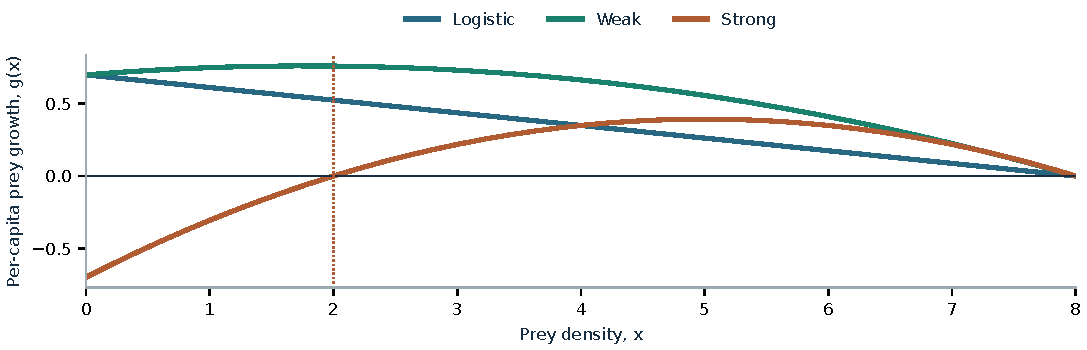
\includegraphics[width=.72\linewidth]{d2/repro/figures/growth.pdf}\end{center}
{\small\textbf{Figure 2.1.} Per-capita prey growth for $r=0.7$, $K=8$, $\alpha=0.225$, and $A=2$. Only strong Allee growth is negative below the threshold $A$.\par}

\clearpage
\subsection*{Equilibria, trajectories, and population removal}
At coexistence set $z=y/\beta$, $s=\beta d/(em)$, and $\kappa=h\beta/d$. The predator equation gives $x=s(1+z)(1+\kappa z)$. Substitution in the prey equation gives
\[
 H(z)=(1+z)g\!\left(s(1+z)(1+\kappa z)\right)-mz=0 .
\]
Each positive root gives one coexistence state. Logistic growth allows at most one. For each Allee law the upper bound is three, counting multiplicity, with rational examples attaining three distinct roots in both competition arms. For example, take $g(x)=1/5+27x/200-x^2/50$, $s=33/76$, and $m=399/800$. For both $\kappa=0$ and $\kappa=32/45045$, the signs of $H$ at $3,7/2,9/2,6$ are $+,-,+,-$. Continuity gives three distinct positive roots in each case. The table uses a separate shared baseline.

\begin{center}\small
\begin{tabular}{@{}llcc@{}}\toprule
Law & Model & Attracting $(x,y)$ & Saddle $(x,y)$\\\midrule
Logistic & M1 & $(5.526,3.110)$ & ---\\
Logistic with competition & M3 & $(5.842,2.038)$ & ---\\
Weak Allee & M0 & $(6.959,4.228)$ & ---\\
Weak Allee with competition & M4 & $(7.109,2.498)$ & ---\\
Strong Allee & M2 & $(6.915,4.194)$ & $(2.466,0.724)$\\
Strong Allee with competition & M5 & $(7.091,2.491)$ & $(2.340,0.469)$\\\bottomrule
\end{tabular}
\end{center}

\begin{center}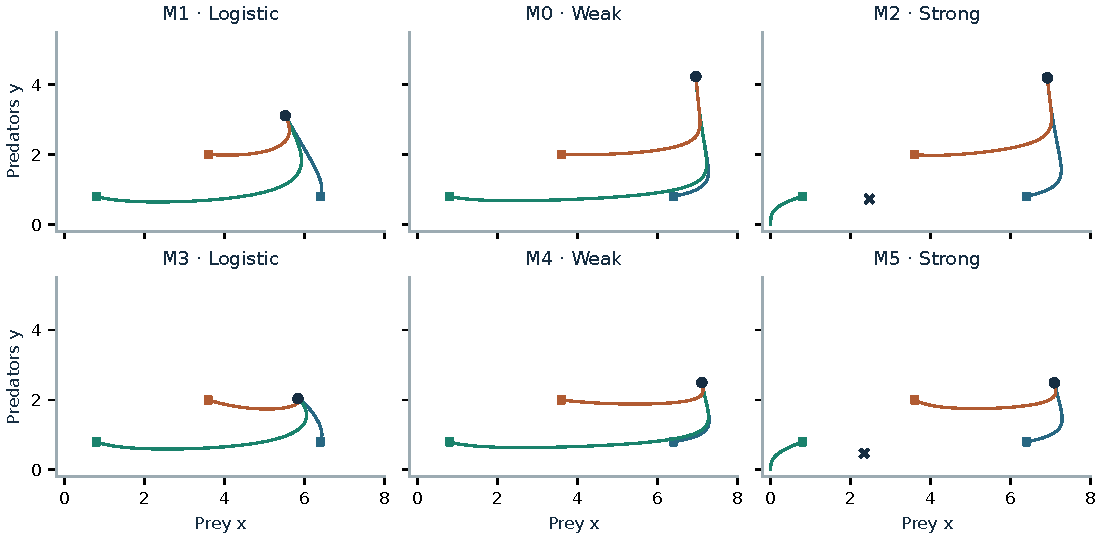
\includegraphics[width=.97\linewidth]{d2/repro/figures/phase.pdf}\end{center}
{\small\textbf{Figure 2.2.} Six models, three common starting states. Squares mark $(6.4,0.8)$, $(0.8,0.8)$, and $(3.6,2)$. Circles mark attracting coexistence states and crosses mark saddles. The table and figure use $r=0.7$, $K=8$, $\alpha=0.225$, $A=2$, $m=0.3$, $\beta=1.2$, $e=0.65$, and $d=0.25$. The lower row uses $h=0.05$.\par}

\textbf{Shocks.} From each model's high-prey attracting equilibrium we removed 5, 25, 60, or 85\% of either species. In 45 of 48 runs both populations recovered to within 2\% of their starting densities and stayed there for at least the last 50 time units of a 600-unit run. After 60\% prey removal, both strong-growth models still started above $A=2$. M2 went extinct from $x=2.766$, while M5 recovered from $x=2.836$ in 17.5 time units. The predator density present after removal helps determine which side of the recovery boundary the system reaches.

\clearpage
\subsection*{Matched competition and held-out prediction}
For the mathematical comparison, we calibrated one growth-rate coefficient per law so that the three models shared $(x_0,y_0)$ at $h=0$. At each later $h$ while the three equilibrium branches remain positive with positive determinant, the strong law has the most predators and the logistic law has the fewest. This comparison concerns the branch connected to the matched starting point. Figure~2.3 also shows how the common interval can end. The choice of matching matters in the wider simulation study. Across 24 matched runs, the weak-minus-logistic contrast in the competition effect on mean late predator density was $-1.401$ at equal $r$ and $+0.355$ when growth rates were matched at $0.6K$.

\begin{center}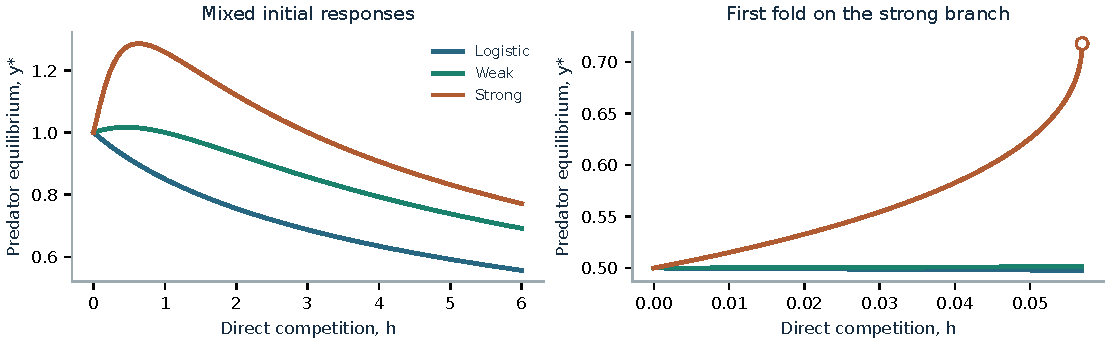
\includegraphics[width=.98\linewidth]{d2/repro/figures/ordering.pdf}\end{center}
{\small\textbf{Figure 2.3.} Predator abundance against competition strength. Left, the common start is $(4,1)$, and at $h=6$ predator densities are $0.5564$ (L), $0.6915$ (W), and $0.7711$ (S). Right, the strong branch reaches a fold at $h\simeq0.056907$ in a separate example with $K=4$.\par}

\textbf{Empirical comparison.} Each fold fitted three chemostat experiments and predicted the fourth. A one-step forecast starts from the previous observation. A free-running forecast starts only once. Scores are the mean of the two species' root mean square errors, each divided by its training standard deviation or by $0.1$ if that deviation is smaller, then averaged equally across four held-out experiments. Lower scores indicate smaller errors.

\begin{center}\small
\begin{tabular}{@{}lrr@{}}\toprule
Model or reference & One-step error & Free-running error\\\midrule
M0 weak & 0.8858 & 1.0420\\
M1 logistic & 0.8849 & 1.0376\\
M2 strong & 0.8990 & 1.0802\\
M3 logistic with competition & \textbf{0.8825} & 1.0582\\
M4 weak with competition & 0.8855 & 1.0621\\
M5 strong with competition & 0.8966 & 1.0978\\
Persistence & 1.0403 & 2.1521\\
Training mean & 1.0370 & \textbf{1.0370}\\
Training drift & 1.0403 & 2.3607\\\bottomrule
\end{tabular}
\end{center}
M3 reduced mean one-step error by 15.2\% relative to persistence and by 0.270\% relative to M1. In all 48 free-running records, the 95th minus the 5th percentile in the final half of the time span was below 5\% of the corresponding training standard deviation. Observed prey minima also exceeded every fitted strong Allee threshold. The records therefore provide no direct observation of a threshold crossing. Data and study design come from Blasius et al., \emph{Nature} 577 (2020), 226--230 \href{https://doi.org/10.1038/s41586-019-1857-0}{(article)} and the \href{https://doi.org/10.6084/m9.figshare.10045976.v1}{public observations}.

\clearpage
\subsection*{Mathematical proof of the matched competition order}
\textbf{Statement.} Fix $K,m,\beta,e,d>0$, choose $0<A<x_0<K$, $\alpha K>1$, $\alpha>0$, and choose $y_0>0$ satisfying $emx_0=d(\beta+y_0)$. Write $q=my_0/(\beta+y_0)$ and $U(x)=(K-x)/(K-x_0)$. Calibrate the three growth rates to
\[
 g_L=qU,\qquad g_W=qU\frac{1+\alpha x}{1+\alpha x_0},\qquad
 g_S=qU\frac{x-A}{x_0-A} .
\]
Assume each initial equilibrium has positive Jacobian determinant. Its local equilibrium branch exists by the implicit function theorem. On any common connected interval starting at zero on which the three branches have positive coordinates and positive determinants, every $h>0$ satisfies
\[
 y_S(h)>y_W(h)>y_L(h),\qquad x_S(h)>x_W(h)>x_L(h)>x_0 .
\]
The right derivatives at zero also satisfy $y_S'(0)>y_W'(0)>y_L'(0)$. Adding negative trace restricts the statement to attracting equilibria.

\textit{Proof.} At a positive equilibrium let $J=\left(\begin{smallmatrix}a&b\\c&-D\end{smallmatrix}\right)$, where
\[
 a=xg'(x),\quad b=-\frac{mx\beta}{(\beta+y)^2},\quad
 c=\frac{emy}{\beta+y},\quad D=y\left(\frac{emx}{(\beta+y)^2}+h\right).
\]
Set $B=-bc>0$ and $\Delta=B-Da$. Differentiating the two zero equations with respect to $h$ gives $J(x',y')^{\mathsf T}=(0,y^2)^{\mathsf T}$. Therefore
\[
 x'=-\frac{by^2}{\Delta}>0,\qquad y'=\frac{ay^2}{\Delta} .
\]
At the common start the three logarithmic growth slopes share the term $-1/(K-x_0)$. The remaining terms are $0$, $\alpha/(1+\alpha x_0)$, and $1/(x_0-A)$, in increasing order, since their last difference is $(1+\alpha A)/[(x_0-A)(1+\alpha x_0)]>0$. The three growth rates agree there, so $a_S>a_W>a_L$. The other Jacobian entries are shared at the start. Subtraction gives
\[
 y_i'(0)-y_j'(0)=\frac{y_0^2B(a_i-a_j)}{\Delta_i\Delta_j}.
\]
This orders the initial derivatives and therefore the predator densities for small $h>0$.

Each branch moves to $x>x_0$, and $g_i(x)=my/(\beta+y)>0$ forces $x<K$. On $(x_0,K)$ the multipliers of $qU(x)$ are $1$, $1+\alpha(x-x_0)/(1+\alpha x_0)$, and $1+(x-x_0)/(x_0-A)$. Hence $g_S>g_W>g_L$ there. A later equality of two predator densities at the same $h$ would force a common prey density through $x=(\beta+y)(d+hy)/(em)$, then equal growth rates through the prey equations. This contradicts the strict growth order. Continuity proves the predator ranking throughout. The same expression for $x$ is strictly increasing in $y$ at fixed $h$, proving the prey ranking.\hfill$\square$

\textbf{An exact example.} For $K=10$, $x_0=4$, $y_0=A=\alpha=m=\beta=1$, $e=2$, and $d=4$, the calibrated growth coefficients are $r_L=5/6$, $r_W=1/6$, and $r_S=5/18$. Substitution gives $y_L'(0)=-1/5$, $y_W'(0)=1/13$, and $y_S'(0)=1$. Competition initially lowers predator density with logistic growth and raises it with either Allee law. The finite theorem ranks the densities even where a branch later changes direction, as in the left panel of Figure~2.3.

\clearpage
\subsection*{Python code and numerical checks}
This Python example uses the matched equilibrium $(4,1)$ on the preceding page. For each growth law it calculates $a=x_0g'(x_0)$, the determinant $\Delta=B-Da$, and the initial predator response $y'(0)=ay_0^2/\Delta$.

\begin{lstlisting}[language=Python,basicstyle=\ttfamily\footnotesize]
from fractions import Fraction as F

x0, y0, K, A, alpha = 4, 1, 10, 1, 1
m, beta, e = 1, 1, 2
q = F(m*y0, beta + y0)
b = -F(m*x0*beta, (beta + y0)**2)
c = F(e*m*y0, beta + y0)
D = F(y0*e*m*x0, (beta + y0)**2)  # h = 0
for extra in (0, F(alpha, 1 + alpha*x0), F(1, x0 - A)):
    a = x0*q*(-F(1, K - x0) + extra)
    determinant = -b*c - D*a
    assert determinant > 0
    print(a*y0**2 / determinant)
\end{lstlisting}
The output, in logistic, weak Allee, and strong Allee order, is $-1/5$, $1/13$, and $1$. The larger numerical check isolated the positive roots of 29 rational examples, checked 12 bifurcation cases, confirmed recovery in 45 of 48 disturbance runs, and recalculated the held-out forecast errors. Across 18 reintegrated trajectories, the largest difference divided by one plus the magnitude of the original coordinate was $2.5\times10^{-8}$.

\subsection*{Lean verification results}
Lean 4.19.0 with Mathlib v4.19.0 checked 47 public declarations. It verified local branch existence from a common equilibrium and the strict order of the initial predator derivatives. It also proved the ordering of both populations on any connected branch segment from that equilibrium where all coordinates and determinants stay positive. For each Allee law, Lean verified the bound of three positive roots, counting multiplicity, and exact examples attaining it with zero and with positive competition. The recovery rates, trajectories, and forecast scores were checked numerically.

\startdirection{3}{Cross-domain prediction}
\section*{Direction 3. Can one predator--prey equation predict outcomes in other biological systems?}

\subsection*{Abstract}
We tested the course equation on five experimental settings in which one population affects another. On a glioma cell line, the equation gave lower mean prediction error than CARRGO, a model for chimeric antigen receptor (CAR) T-cell therapy. A model that tracks stages of infection was more accurate in 11 of 12 four-hour bacteriophage tests. A separate leukemia dataset measured both interacting populations. Fitting the equation to both populations recovered all twelve early T-cell increases, but more than doubled the mean error for the target cells. A mathematical comparison explains how an accurate target forecast can depend only weakly on the modeled interaction.

\subsection*{Results}
\textbf{What transferred between systems.}
We kept the original two equations and fitted their seven positive coefficients using the training conditions in each assay. Writing $x$ for the target and $y$ for the consumer gives
\[
 \dot x=xg(x)-F(x,y),\qquad \dot y=eF(x,y)-dy,\qquad
 g(x)=r(1-x/K)(1+\alpha x),\quad F(x,y)=\frac{mxy}{\beta+y}.
\]
Here $g$ is the course model's per-capita prey growth law. Per-capita growth initially increases with density when $\alpha K>1$. The term $F$ removes targets, and the same flux contributes $eF$ to consumer growth. In the cell assays, the target is a tumor cell population and the consumer represents T cells. In the phage assays, $x$ represents bacteria and $y$ represents phage.

\textbf{What counted as a successful prediction.}
Each test held out a whole dose, input level, or population ratio. We scored errors on the measurement scale of that assay. Cell Index (CI) measures electrical impedance, optical density (OD) measures a culture's effect on transmitted light, and the leukemia assay reports marker-positive cell counts. Root-mean-square error (RMSE) is the square root of the mean of the squared differences between predictions and observations. Smaller values indicate closer predictions. Means across conditions give each held condition equal weight.

\textbf{Which target forecasts relied on the consumer?}
For each ecological fit to the cell-line data, we kept all coefficients and the starting target level fixed and set the starting consumer to zero. In the six primary PBT138 tests, this changed the predicted target by a maximum of 2.20--2.54 CI on the held time grids. In five of six HT1080 tests the maximum change was below 0.000052 CI. The sixth reached 0.07934 CI. The same equation therefore assigned very different roles to the interacting population.

\textbf{Which forecast was tested?}
The main comparisons transferred the equation and fitted its coefficients to training conditions in each assay. Separate tests froze those coefficients before forecasting a different cell line or acquisition. The leukemia study added a second measured population, allowing the target forecast and the consumer forecast to be scored separately.

\clearpage
\subsection*{Figures and tables}
\subsubsection*{Held target measurements across assays}
\begin{center}
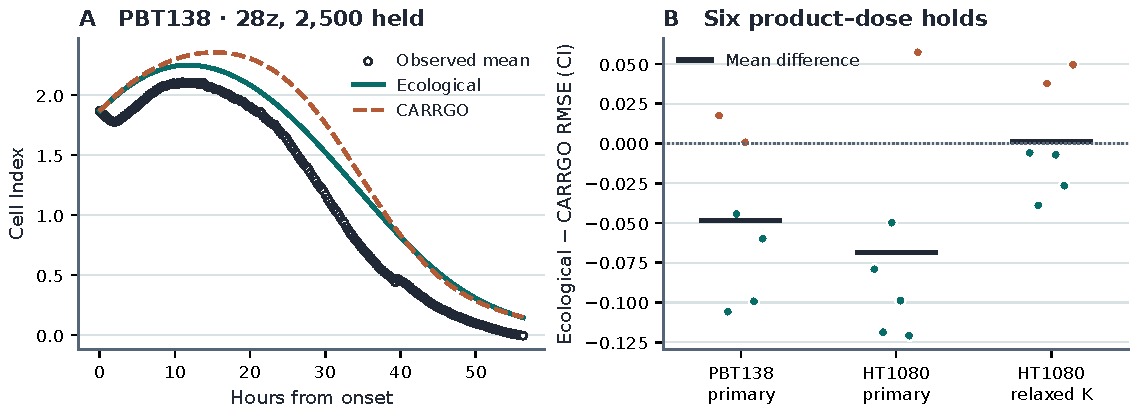
\includegraphics[width=.93\linewidth]{d3/figures/cart_held.pdf}
\captionof{figure}{Cell Index after a held dose. At left, points and lines refer to one held PBT138 condition. At right, each point is an ecological-minus-CARRGO RMSE difference for one of six conditions. A negative value favors the ecological equation.}
\end{center}
In PBT138, the ecological equation won four of six held conditions, with mean errors of 0.288 CI for ecology and 0.336 CI for CARRGO. For HT1080, the untreated controls reached 10.118 CI, above the original capacity ceiling of 10. Raising only that ceiling changed the mean errors from 0.3052 and 0.3736 CI to 0.1993 and 0.1978 CI, respectively. Freezing the coefficients across cell lines gave ecological and CARRGO errors of 0.587 and 0.519 CI from PBT138 to HT1080, and 1.700 and 1.015 CI in reverse, over 24 hours.

\begin{center}
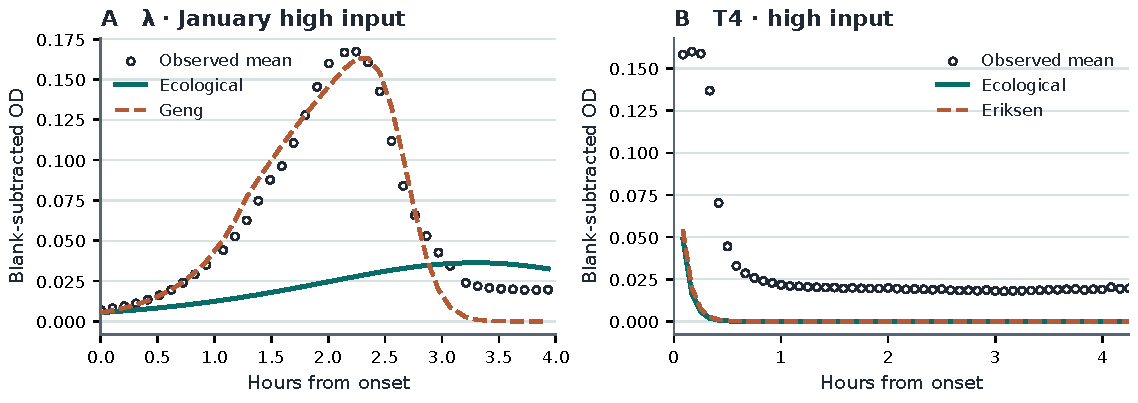
\includegraphics[width=.93\linewidth]{d3/figures/phage_held.pdf}
\captionof{figure}{Optical density at a held high input in two independent assays. Points are mean observations and curves are model predictions. The January $\lambda$ assay used Geng's infection-stage model as the comparator. The T4 assay used Eriksen's resource model.}
\end{center}
Geng's model had lower four-hour error in 11 of 12 held inputs across four $\lambda$ acquisitions. On independent T4 data, ecology won two of three inputs over 4.25 hours and one of three over the first hour. A separate transfer experiment froze January's $\lambda$ parameters and scored 18 positive conditions on three later dates. Ecology then had lower mean four-hour error (0.0628 vs.\ 0.0747 OD), although it won only eight individual comparisons. The average and the number of wins give different information about the size of the errors.

\clearpage
\subsubsection*{Predicting both populations with one parameter vector}
The LT6 leukemia assay recorded CD33-positive targets and total CD3-positive T cells. Each of two target genotypes, wild type (WT) and TP53 knockout (KO), had six treated ratios. For each held ratio, we fitted on the other five ratios of the same genotype and included target values from the untransduced controls. One vector then predicted both markers at days 6, 10, and 16 from the held condition's measured day-3 counts. The twelve comparisons describe one acquisition and share training data.

\begin{center}
\captionof{table}{Primary LT6 results. The two error columns give mean RMSE across the twelve held conditions in dilution-corrected cell counts. The last column counts correct predictions of the observed CD3 increase from day 3 to day 6.}
\small
\begin{tabular}{@{}lrrr@{}}\toprule
Model and fitting rule & CD33 RMSE & CD3 RMSE & Early rises \\\midrule
Ecology, target only & 81,634 & 6,099 & 0/12 \\
Ecology, 5\% target-loss band & 83,611 & 5,025 & 10/12 \\
Ecology, equal-weight joint fit & 197,580 & 4,990 & 12/12 \\
CARRGO, equal-weight joint fit & 177,505 & 5,095 & 11/12 \\
Shah Beddington--DeAngelis, joint fit & 134,300 & 4,594 & 12/12 \\
Growth model and constant CD3 & 81,648 & 5,019 & 0/12 \\
Growth model and day-specific CD3 & 81,648 & 2,039 & 12/12 \\\bottomrule
\end{tabular}
\end{center}
Equal-weight training used the sum of the two normalized marker losses. The 5\% rule selected for lower CD3 training loss among candidates within 5\% of the lowest CD33 training loss found. The day-specific CD3 reference multiplied the held starting count by the median change factor among training ratios at each forecast day. It gave a lower CD3 RMSE than the joint ecological fit in all twelve conditions.

\begin{center}
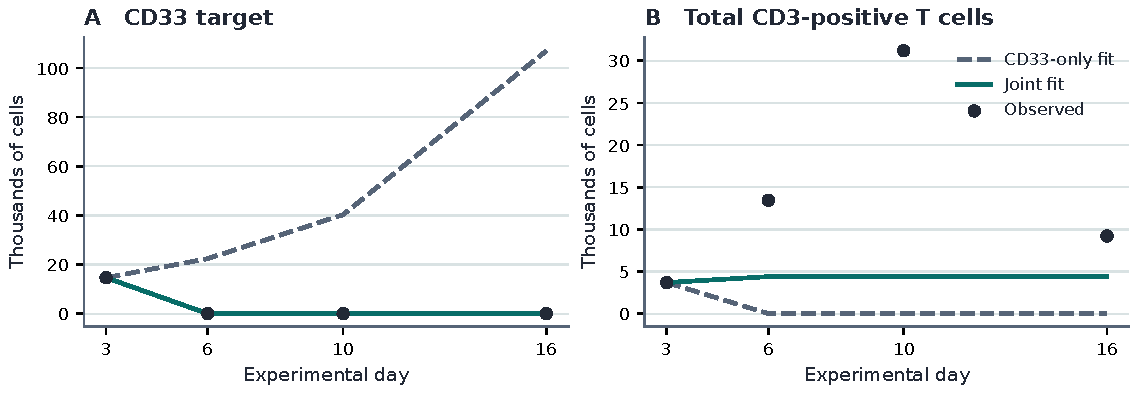
\includegraphics[width=.94\linewidth]{d3/figures/aml_case.pdf}
\captionof{figure}{Held wild-type 1:16 condition. Both fits used the same day-3 measurements. The joint fit predicted the rapid loss of CD33-positive targets closely (RMSE 21.7 counts). It predicted about 4,393 CD3-positive cells on day 10, when 31,180 were observed.}
\end{center}
At fixed joint coefficients, retaining the consumer improved CD33 error relative to setting its initial value to zero in three of twelve conditions. Across all twelve, mean CD33 RMSE was 197,580 with the consumer and 131,587 without it. Total CD3 includes cells whose functional activity was unmeasured.

\clearpage
\subsection*{Mathematical proof}
\textbf{How much can the consumer change a target forecast?}
Take positive coefficients and initial values $x_0,y_0>0$. On $[0,T]$, compare the positive interacting solution $(x,y)$ with the solution $(X,0)$ from $(x_0,0)$ using the same coefficients. Set
\[
 M=\max(K,x_0),\quad A=\alpha K,\quad
 \gamma=d-\frac{emM}{\beta},\quad L=\frac{r\max(A-1,0)^2}{8A}.
\]
If $\gamma>0$, then for $0\le t\le T$,
\[
 0\le X(t)-x(t)\le M(1-e^{-Z_T}),\qquad
 Z_T=e^{LT}\frac{m}{\gamma}\log(1+y_0/\beta).
\]

\textit{Proof.}
Write $h(y)=my/(\beta+y)$. On a regular trajectory the consumer satisfies
$\dot y=y\{emx/(\beta+y)-d\}$. Integrating this linear equation in $y$ along the trajectory shows that a zero initial consumer remains zero. Its associated target therefore solves $\dot X=Xg(X)$. A positive initial state remains positive on the solution interval by the same factorization for each population. At $M$ the two target derivatives are nonpositive. Since $\dot x\le xg(x)$, scalar comparison gives $0<x\le X\le M$.

It follows that $\dot y/y\le-\gamma$ and $y(t)\le y_0e^{-\gamma t}$. Monotonicity of $h$ gives
\[
 \int_0^t h(y(s))\,ds
 \le \int_0^\infty \frac{my_0e^{-\gamma s}}{\beta+y_0e^{-\gamma s}}\,ds
 =\frac{m}{\gamma}\log(1+y_0/\beta).
\]
The derivative of $g(x)$ with respect to $\log x$ is the quadratic
$xg'(x)=r[(\alpha-1/K)x-2\alpha x^2/K]$. Its supremum for $x>0$ is $L$. The vertex gives $r(A-1)^2/(8A)$ for $A>1$, and the supremum is zero as $x\downarrow0$ for $A\le1$. Hence
$z=\log(X/x)\ge0$ satisfies $\dot z=g(X)-g(x)+h(y)\le Lz+h(y)$.
Integrating from $z(0)=0$ gives $z(t)\le Z_T$.
Finally $X-x=X(1-e^{-z})\le M(1-e^{-Z_T})$.

\textbf{Why this protects the target-error rankings.}
On a common grid of $n\ge1$ observations $o$, write $E(u)=\|u-o\|_2/\sqrt n$.
The reverse triangle inequality gives
$|E(u)-E(v)|\le\|u-v\|_2/\sqrt n\le\max_i|u_i-v_i|$.
Thus a strict error gap to a comparator survives any smaller uniform change in the forecast. On the 13-day LT6 window, the largest target-only displacement bounds were 143.16 counts under primary bounds and 37.20 under expanded bounds. The smallest comparator gaps were 898.93 and 1,109.93 counts, respectively. All $12\times2\times3=72$ rankings therefore survived removal of the consumer. The three comparators were CARRGO, Shah Beddington--DeAngelis, and the fixed-dose model. For primary joint ecological fits, $\gamma>0$ failed in all twelve conditions. Their fixed-coefficient comparisons used direct numerical integration.

\begin{center}
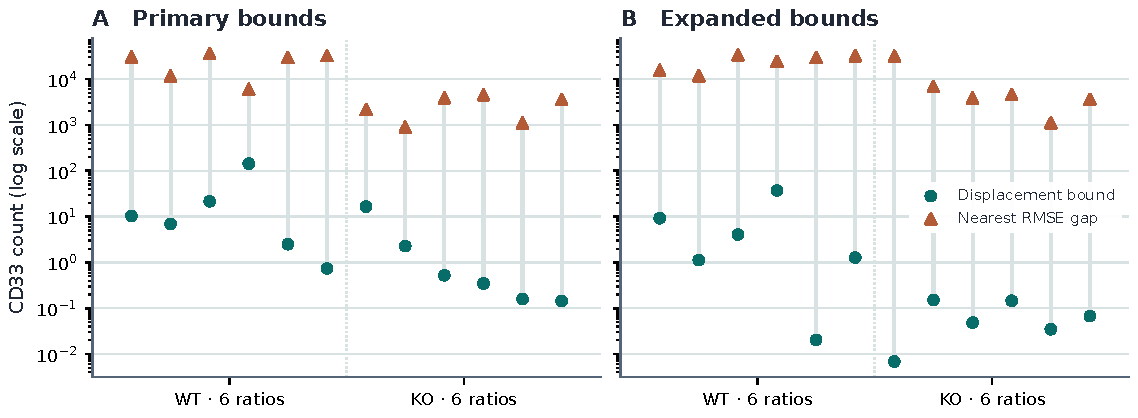
\includegraphics[width=.84\linewidth]{d3/figures/ablation_certificate.pdf}
\captionof{figure}{Each circle gives the target displacement bound for one of the twelve held LT6 ratios. The triangle above it gives the smallest RMSE gap to any comparator. The two panels use the same condition order and report dilution-corrected CD33 counts on a logarithmic scale.}
\end{center}

\clearpage
\subsection*{Python code}
This example scores the equal-weight joint forecast for the held wild-type 1:16 condition in Figure~3.3. Inputs are dilution-corrected counts on days 3, 6, 10, and 16. Forecast values are rounded for display. Day 3 initializes the forecast, so the error uses only the last three dates.

\begin{lstlisting}[language=Python,basicstyle=\ttfamily\footnotesize]
from math import sqrt
from statistics import mean

observed_cd33 = (14656.2, 37.6, 0.0, 0.0)
forecast_cd33 = (14656.2, 0.0, 0.0, 0.0)
observed_cd3 = (3687.6, 13463.2, 31179.5, 9212.1)
forecast_cd3 = (3687.6, 4393.245, 4393.228, 4393.201)

def rmse(observed, forecast):
    pairs = zip(observed[1:], forecast[1:])
    return sqrt(mean((o - p)**2 for o, p in pairs))

print(round(rmse(observed_cd33, forecast_cd33), 1))
print(round(rmse(observed_cd3, forecast_cd3), 1))
print(forecast_cd3[1] > forecast_cd3[0] + 1e-7)
\end{lstlisting}
The outputs are 21.7 CD33 counts, 16,562.9 CD3 counts, and \texttt{True} for the early rise. The averages in Table~3.1 give equal weight to each of the twelve held conditions.

\subsection*{Lean verification results}
Lean 4.19.0 with Mathlib v4.19.0 checked 22 public declarations. For regular solutions on a finite interval, it verified that zero initial consumer density stays zero and that the target then follows its scalar growth equation with the original parameters and initial target. It also verified the conditional upper bound on consumer density, the RMSE inequality, and the resulting sufficient condition for preserving an error ranking.

Two proofs verify that the twelve genotype--ratio pairs are distinct and that the observed CD3 count rose from day 3 to day 6 in each. Both proofs use no axioms. Python matched the 24 counts to the published LT6 observations. The preceding page derives the full target displacement bound and applies it to 72 forecast comparisons.

\newcommand{\repo}{https://github.com/lijincheng494gmail/project-3h-research-extensions}
\newcommand{\asset}[2]{\href{\repo/releases/download/v1.0/#1}{#2}}
\newcommand{\sourceLink}[2]{\href{https://doi.org/#1}{#2}}

\subsection*{Research papers and reproducibility}
\textbf{Code and data.}
\asset{Project_3H_Research_Extensions_Source.zip}{Download the reproducibility package}
\quad
\href{\repo}{Browse the public GitHub repository}.

\textbf{Project manuscripts.}
The GitHub release provides the research drafts.
\begin{itemize}[leftmargin=1.2em,topsep=2pt,itemsep=1pt]
\item Direction 1.
\asset{Direction_1_Five_Model_Comparison.pdf}{Five-model comparison}
and \asset{Direction_1_Enrichment_Criterion.pdf}{reciprocal-curvature criterion}.
\item Direction 2.
\asset{Direction_2_Six_Model_Comparison.pdf}{Six-model comparison},
\asset{Direction_2_Competition_Ordering.pdf}{competition ordering},
and \asset{Direction_2_General_Comparison.pdf}{general comparison theorem}.
\item Direction 3.
\asset{Direction_3_Cross_Domain_Prediction.pdf}{Cross-domain prediction and dual readouts}.
\end{itemize}

\textbf{Published studies and data.}
\sourceLink{10.1007/s11538-008-9368-4}{Haque (2009)},
\sourceLink{10.1016/j.mbs.2011.07.003}{Haque (2011)},
\sourceLink{10.1007/s00285-010-0332-1}{Wang et al. (2011)},
\sourceLink{10.1016/j.ecocom.2012.01.002}{Sen et al. (2012)},
\sourceLink{10.3934/dcdsb.2013.18.2283}{Gao and Li (2013)}, and
\sourceLink{10.58997/ejde.2023.17}{Feng and Li (2023)}
give the mathematical background.
\sourceLink{10.1038/s41586-019-1857-0}{Blasius et al. (2020)}
and their \sourceLink{10.6084/m9.figshare.10045976.v1}{Figshare data}
supply the ecology comparison.

\sourceLink{10.1098/rsif.2019.0734}{Sahoo et al. (2020)},
\sourceLink{10.1038/s41467-024-51913-6}{Geng et al. (2024)},
\sourceLink{10.1371/journal.pone.0216292}{Rajnovic et al. (2019)},
\sourceLink{10.1038/s41598-020-59635-7}{Eriksen et al. (2020)}, and
\sourceLink{10.1186/s12935-026-04419-8}{Shah et al. (2026)}
supply the cross-domain studies and comparators.
The LT6 marker counts are in the \sourceLink{10.5281/zenodo.12823159}{Zenodo archive}.

\end{document}
